\section{Versuchsaufbau/-durchführung}
Der verwendete Aufbau ist in Abbildung \ref{fig: aufbau} schematisch dargestellt. Die Vakuumpumpe ist als Handpumpe
realisiert, als Lichtquelle dient ein Helium-Neon-Laser. Zur Justage des Aufbaus wird zunächst ein Blatt Papier vor das Photoelement gehalten,
auf dem das Interferenzbild betrachtet werden kann. Mit zwei Rändelschrauben wird der eine Spiegel so justiert,
dass die beiden hellsten erkennbaren Interferenzmaxima
aufeinander liegen. In diesem Fall verlaufen die beiden Teilbündel genau parallel. Das Hauptmaximum des kreisförmigen Intefrenzbildes
liegt auf dem Photoelement, das in Verbindung mit einem Verstärker und einem elektronischen Zählwerk zur Aufzeichnung der Anzahl
der auftretenden Maxima $z$ dient.\\
Zur Messung der Wellenlänge des Laserlichtes wird der Synchronmotor und das Zählwerk zeitgleich gestartet. Der Motor verschiebt einen
der beiden Spiegel um eine Strecke $\Delta d$, die an einer Mikrometerschraube abgelesen werden kann. Mit den Wertepaaren ($z$, $\Delta d$) kann
die Wellenlänge bestimmt werden. Der Prozess wird zehn mal durchgeführt. \\
Weiter sollen die Brechungsindices von Luft und Kohlenstoffdioxid experimentell bestimmt werden. Hierzu  wird mit der Pumpe zunächst ein Unterdruck
in der Messzelle erzeugt, der anschließend
durch das Öffnen eines Ventils (zur Umgebung bzw. zu einer Druckgasflasche) wieder ausgeglichen wird. Während dieses Vorgangs wird wiederum die
Anzahl der Intensitätsmaxima aufgezeichnet. Auch dies wird jeweils zehn mal wiederholt. Für die Brechungsindices gilt unter Annahme einer konstanten
Temperatur
\begin{equation}
  \label{eq: brechungsindex}
  n = 1 + \Delta n \frac{p_0}{p - p'} \overset{\eqref{eq: maxima_brechungsindex}}{=} 1 + \frac{z \lambda}{2b} \frac{p_0}{p - p'} .
\end{equation}
Hierbei entspricht $p_0$ dem Atmosphärendruck und $p - p'$ der Druckdifferenz vor und nach dem Druckausgleich. Für $p_0$ wird der Wert $\SI{1.0132}{\bar}$ angenommen,
die anderen beiden Größen werden mit Hilfe eines Barometers ausgemessen.
\begin{figure}
  \centering
  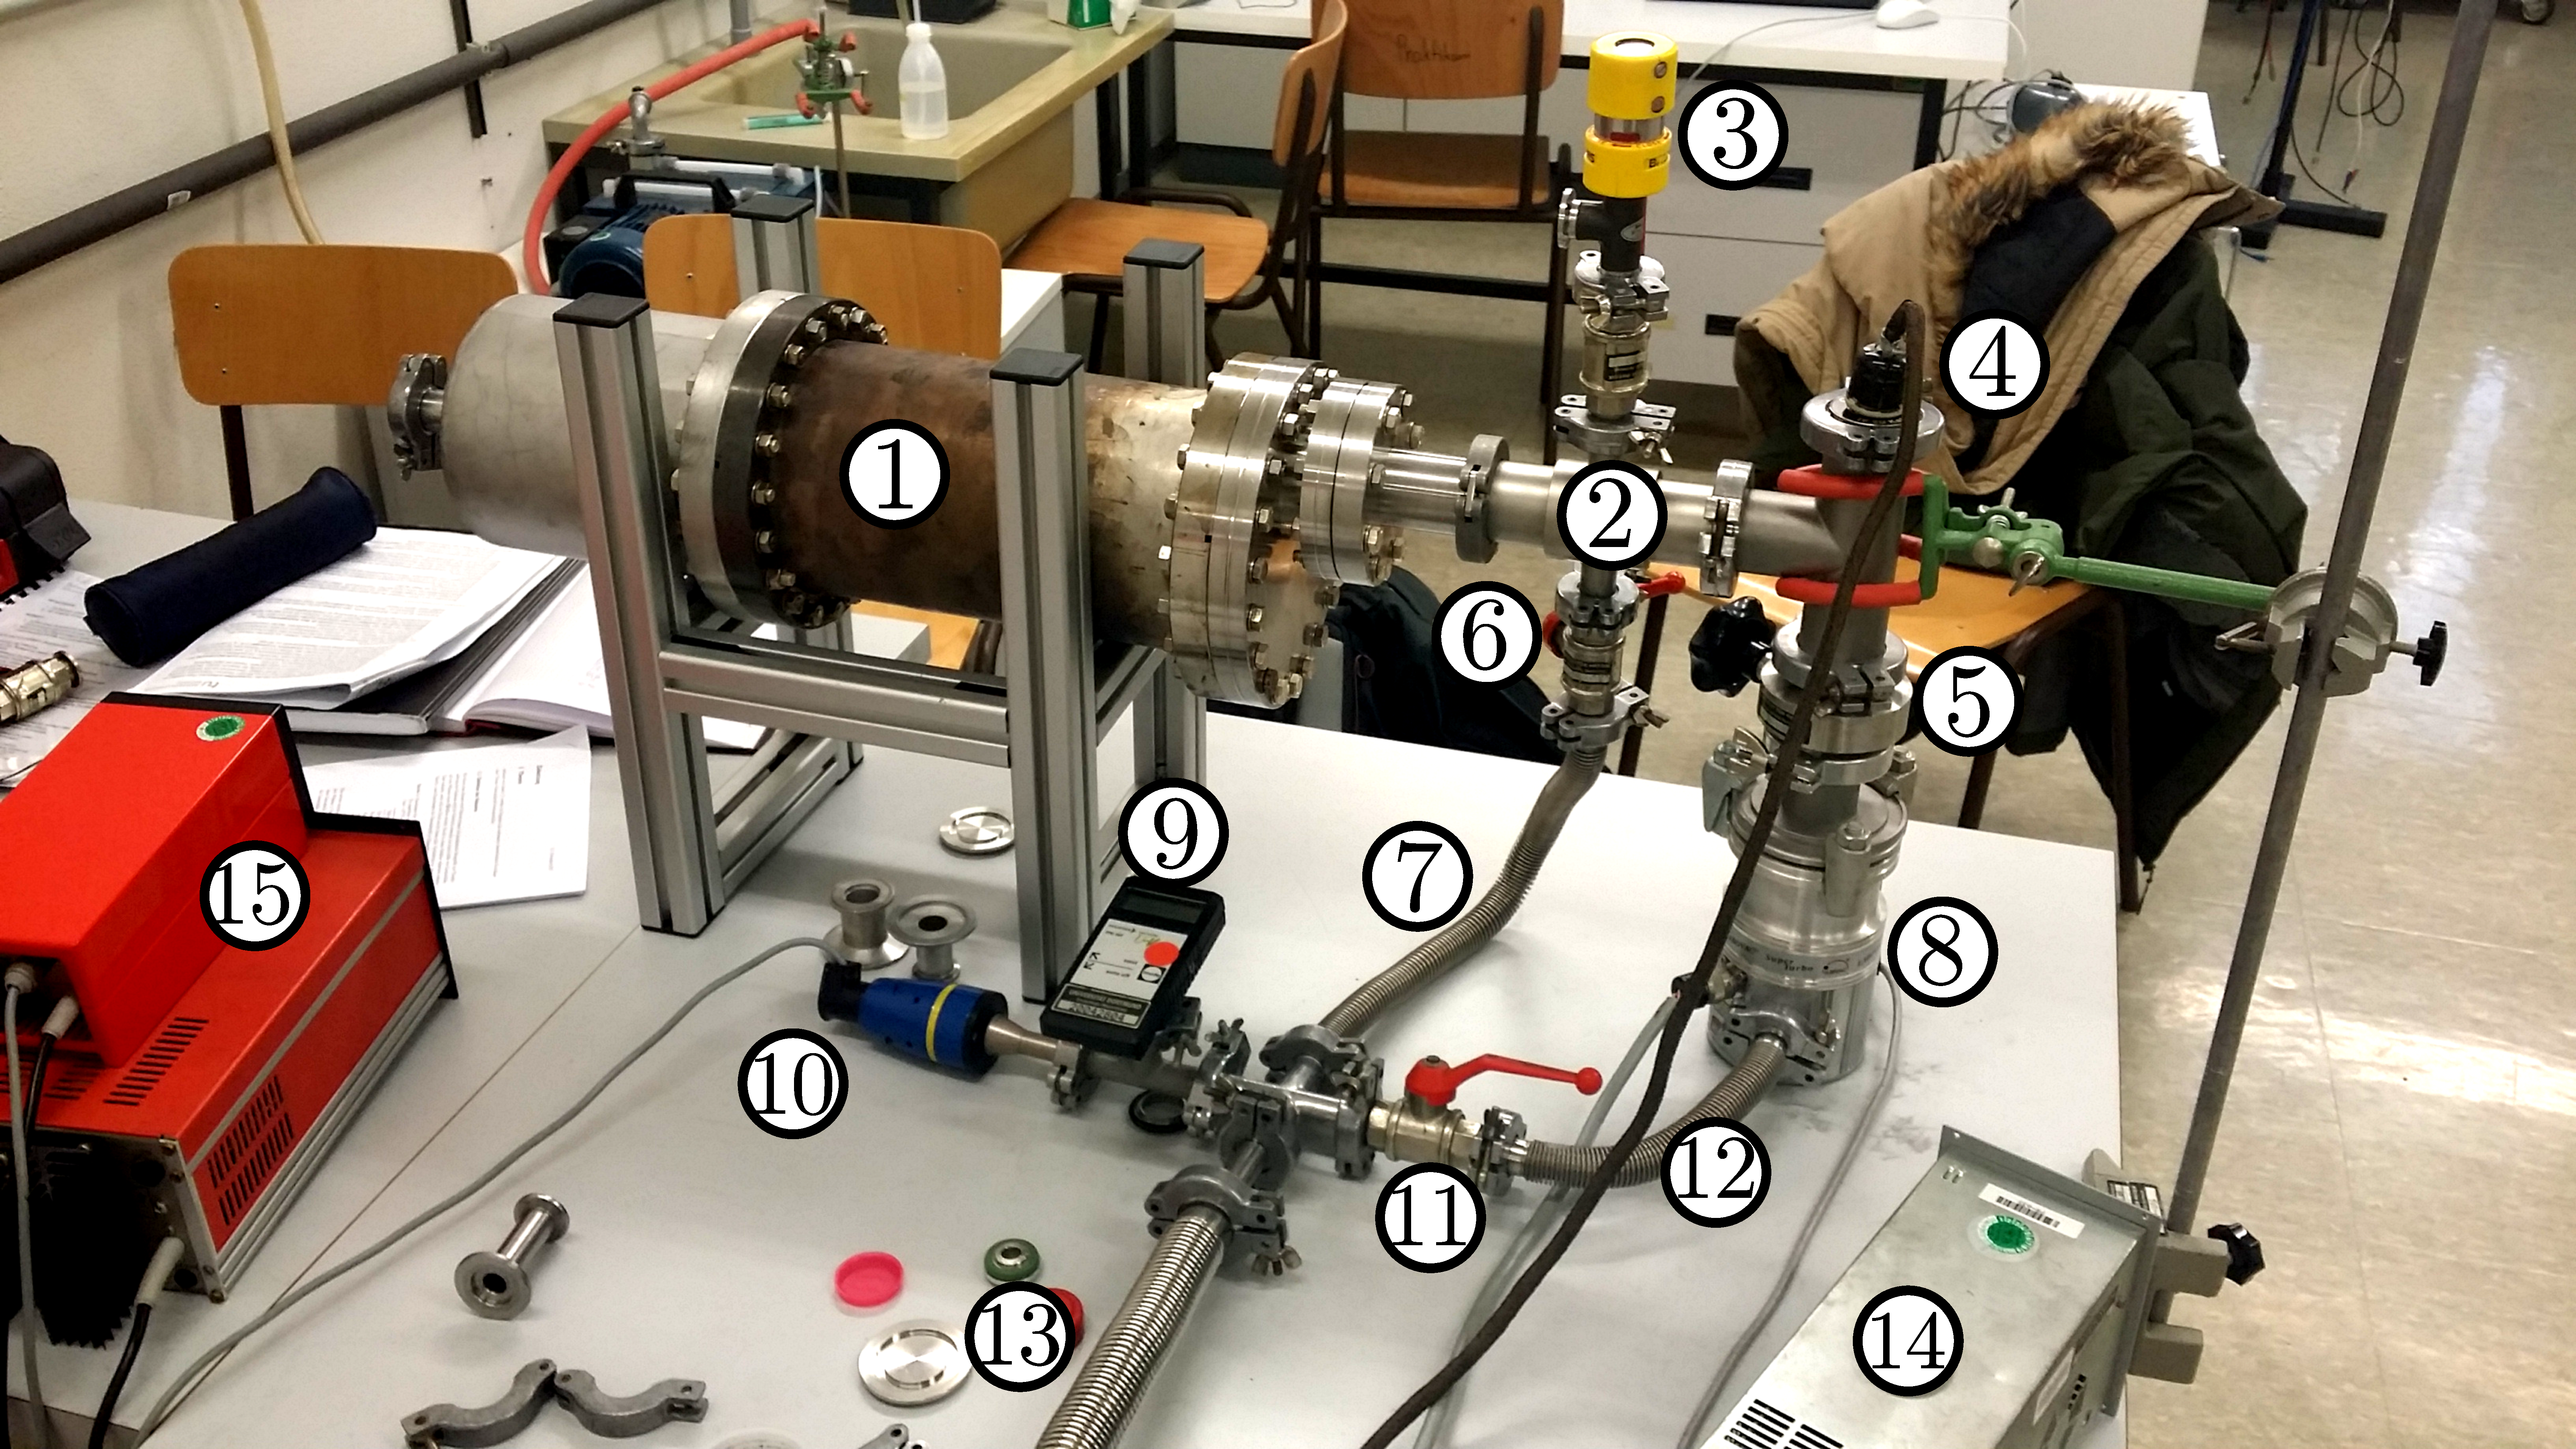
\includegraphics[width = 0.7\textwidth]{table/aufbau.png}
  \caption{Aufbau auf Grundlage des Michelson-Interferometers \cite{anleitung401}.}
  \label{fig: aufbau}
\end{figure}
